% ЕМТ 2018, VI клас — точен LaTeX препис от официалните файлове в Klasirane.com.
% Условия: https://klasirane.com/api/competitions/EMT/All/2018/6%20%D0%BA%D0%BB/probs
% SHA-256 (условия): a12eaed98a21fb1e2622e6c7c0ac5309ef3881cdc25629b01b9baf59fe229a4b
% Решения: https://klasirane.com/api/competitions/EMT/All/2018/6%20%D0%BA%D0%BB/sol
% SHA-256 (решения): 8d7e51ec5837a93a07a798878e266fee5a37e2948b82fd85bd122fc280580388
% Точковите оценки, правописът, формулните нередности и непълнотите са запазени от източника.

Задача 6.1. Намерете числото $\dfrac{X}{0,01}+\dfrac{Y}{Z}$, където

$$Y=5,25:1\dfrac{1}{2}+1,5:3\dfrac{3}{4}.2\dfrac{1}{2}+\left(1\dfrac{1}{7}-\dfrac{23}{49}\right):\dfrac{22}{147},$$

$$Z=2:3\dfrac{1}{5}+3\dfrac{1}{4}:13:\dfrac{2}{3}-\left(2\dfrac{5}{18}-\dfrac{17}{36}\right).\dfrac{18}{65},$$

а $X$ е неизвестното число от равенството:

$$0,125.X:\left(\dfrac{19}{6}-\dfrac{21}{10}\right):8\dfrac{7}{16}=\dfrac{\left(1\dfrac{4}{9}-\dfrac{17}{21}\right).0,7}{0,675.2,4-0,02}.$$

Решение. За намиране $X=20$ – 4 точки

За намиране $Y=9$ – 2,5 точки (по 0,5 точки за всяко действие – умножение или деление)

За намиране $Z=0,5$ – 2,5 точки (по 0,5 точки за всяко действие – умножение или деление)

За намиране $100.X+\dfrac{Y}{Z}=2018$ - 1 точка

Задача 6.2. Сега аз съм на два пъти повече години отколкото Иван беше, когато аз бях на неговата възраст. Сега сборът от годините ни е 42. На колко години е сега всеки от нас?

Решение. Нека говорещият е на $2x$ години. Тогава Иван е на $42-2x$ години. Говорещият е бил на възрастта на Иван преди $2x-(42-2x)=4x-42$ години. Тогава възрастта на Иван е била $42-2x-(4x-42)=84-6x$. От условието имаме: $x=84-6x\Rightarrow x=12$

Оценяване: Подходящо означаване (1т.). Израз за годините на Иван сега (1т.). Израз за изминалите години (3т.). Израз за годините на Иван преди (1т.). Съставяне на уравнение (2т.). Отговор (2т.).

Всяко друго вярно решение се оценява с пълен брой точки

Задача 6.3. Да се намерят шест естествени числа такива, че сумите на всеки пет от тях са 2014, 2015, 2016, 2017, 2018 и шестата сума съвпада с една от изброените.

Решение. Нека сбора на шестте числа е $S$, а числата са $a$, $b$, $c$, $d$, $e$ и $f$. Тогава ще имаме, че $S-a=2014$, $S-b=2015$, $S-c=2016$, $S-d=2017$, $S-e=2018\Rightarrow d=e+1$, $c=e+2$, $b=e+3$, $a=e+4\Rightarrow a+b+c+d+e=5e+10\Rightarrow$ се дели на $5\Rightarrow$

$$5e+10=2015\Rightarrow e=401\text{ и }a=405,\ b=404,\ c=403,\ d=402.$$

Тъй като има само една сума по-малка от 2015, тогава трябва да се повтаря 404л

Оценяване: Подходящо означаване (2т.). Достигане до извод, че има пет последователни числа (2т.). Извод за делимост на 5 (2т.). Откриване на петте последователни числа (2т.). Откриване на повтарящото се число (2т.).

Всяко друго вярно решение се оценява с пълен брой точки

Задача 6.4. На страните $BC$ и $CA$ на $\triangle ABC$ са избрани съответно точки $P$ и $Q$, като $BP:PC=2:1$ и $AQ:QC=1:2$. Точките $M$ и $N$ са средите съответно на отсечките $AP$ и $BQ$. Ако лицето на четириъгълника $ABPQ$ е равно на 2018 кв. см., намерете лицето на $\triangle CMN$.

Решение. Лицето на $\triangle ABC$ ще означим с

Тогава

$$S_{BNC}=\dfrac{1}{2}S_{BQC}=\dfrac{1}{2}.\dfrac{2}{3}S_{ABC}=\dfrac{1}{3}S_{ABC}.$$

Аналогично

$$S_{CMQ}=\dfrac{2}{3}S_{AMC}=\dfrac{2}{3}.S_{MBQ}\dfrac{1}{2}S_{APC}=\dfrac{1}{9}S_{ABC}$$

и $S_{BMC}=\dfrac{1}{2}S_{ABC}\Rightarrow S_{ABMQ}=S_{ABC}-S_{BMC}-S_{CMQ}=\dfrac{7}{18}S_{ABC}\Rightarrow S_{MBQ}=S_{ABMQ}-S_{ABQ}=\dfrac{1}{18}S_{ABC}\Rightarrow S_{MNQ}=\dfrac{1}{36}S_{ABC}$. Откъдето получаваме, че $S_{CMN}=\dfrac{7}{36}S_{ABC}=\dfrac{1}{4}S_{ABPQ}=504,5$ кв. см.

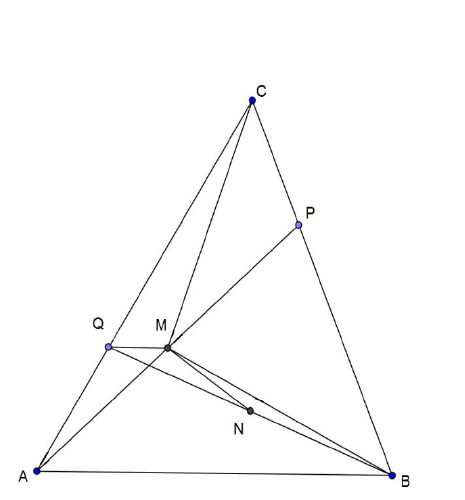
\includegraphics[max width=\textwidth, alt={Чертежът към решението с точките A, B, C, M, N, P и Q}, center]{assets/6-4-solution-figure.png}

Оценяване: За верен чертеж 1 т.

$S_{BNC}=\dfrac{1}{3}S_{ABC}$ (1т.), $S_{CMQ}=\dfrac{1}{9}S_{ABC}$ (2т.) и $S_{BMC}=\dfrac{1}{2}S_{ABC}$ (1т.) $\Rightarrow S_{ABMQ}=\dfrac{7}{18}S_{ABC}$ (1 т.) $\Rightarrow S_{MBQ}=\dfrac{1}{18}S_{ABC}$ (1т.) $\Rightarrow S_{MNQ}=\dfrac{1}{36}S_{ABC}$ (1т.).

Откъдето получаваме, че $S_{CMN}=\dfrac{7}{36}S_{ABC}=\dfrac{1}{4}S_{ABPQ}=504,5$ кв. см. (2т.)

Всяко друго вярно решение се оценява с пълен брой точки
